\section{Datenselektion}
\label{ds}

Opta Sports erfasst in einem Fußballspiel zwischen 1600 und 2000 verschiedene Events (z.B. Pässe, Schüsse, Fouls, uvm.), aus denen eine geeignete Datenmenge für die Funktionsmodellierung ausgewählt werden muss. Zunächst werden die im \gls{xml}-Format vorliegenden Daten eines Spieles für eine bessere Weiterverarbeitung in ein \gls{json}-Format geparst. Über die in \vref{opta} beschriebenen \textsf{Type-IDs} und \textsf{Qualifiers} können die relevanten Schüsse aus dieser großen Datenmenge selektiert werden. Aus der \vref{tab:events} lassen sich alle Schussversuche innerhalb eines Spiels identifizieren, wobei die Zieldaten nur Schüsse beinhalten dürfen, die während des \glqq freien\grqq~Spiels abgeben wurden, nicht aus Eigentoren resultieren und die nicht geblockt wurden (vgl. \vref{tab:anf}). Die Eliminierung solcher Schüsse erfolgt durch die in \vref{tab:quali} aufgelisteten Qualifier. Die Eigentore wurden nicht von vornherein ausgeschlossen und konnte erst durch die Visualisierung aller Torerfolge in \vref{owngoals} ausgeschlossen werden, da diese sonst eine verfälschte Wahrscheinlichkeit für einen Torerfolg aus dieser Position widerspiegeln.\enlargethispage{2\baselineskip} Aufgrund der Qualifier ist es somit möglich, Schüsse wie das \glqq Eigentor des Jahres\grqq\seFootcite{Vgl.}{}{FrankfurterAllgemeineZeitung.2014} von C. Kramer aus 45 Metern Entfernung von der Berechnung auszuschließen.

\begin{sidewaysfigure}[H]
\centering
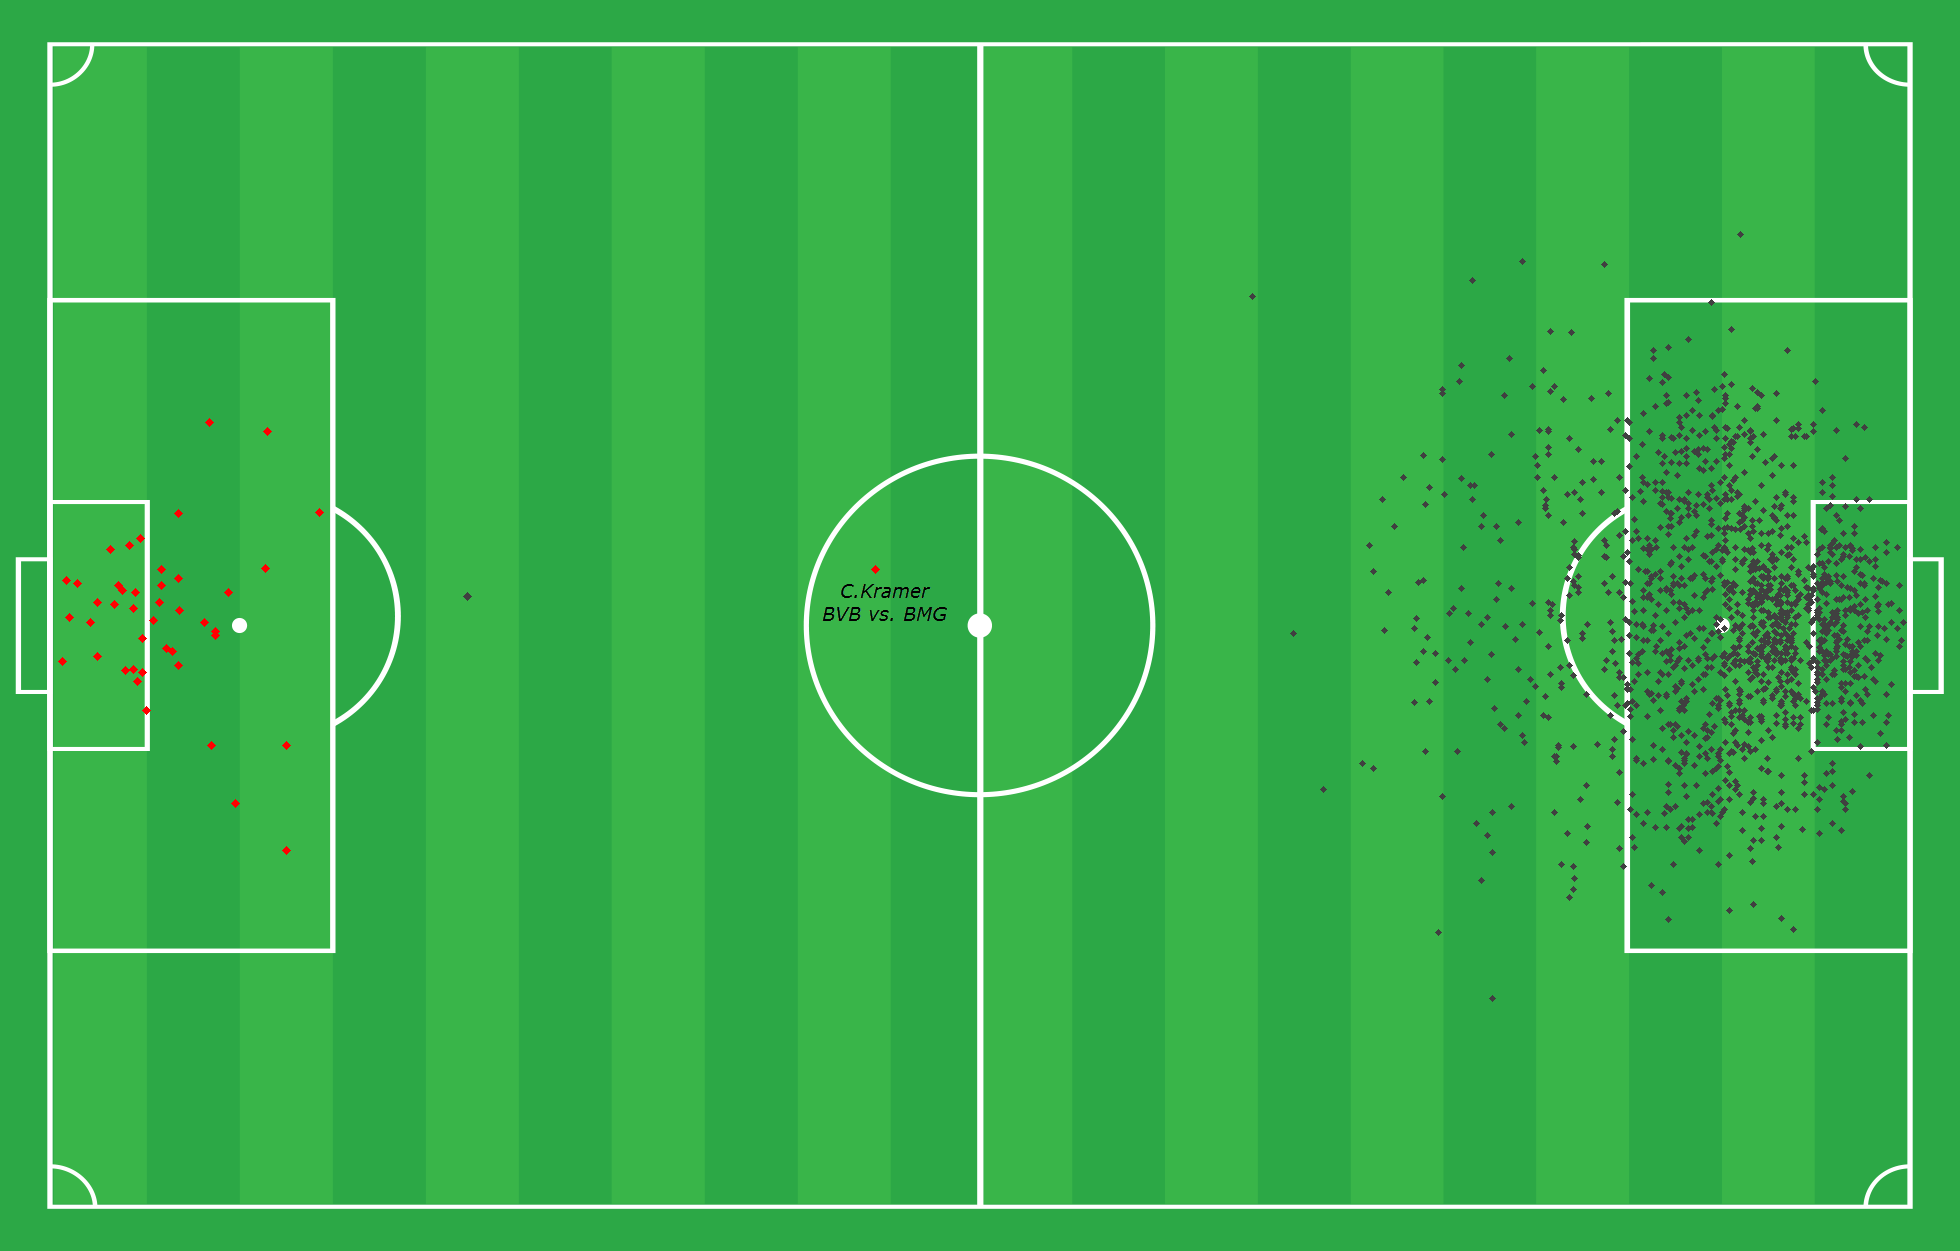
\includegraphics[scale=0.4]{se-wa-jpg/owngoals}
\caption[Ausschluss der Eigentore]{Ausschluss der Eigentore (rote Punkte) }
\label{owngoals}
\end{sidewaysfigure}

%\begin{figure}
%\centering
%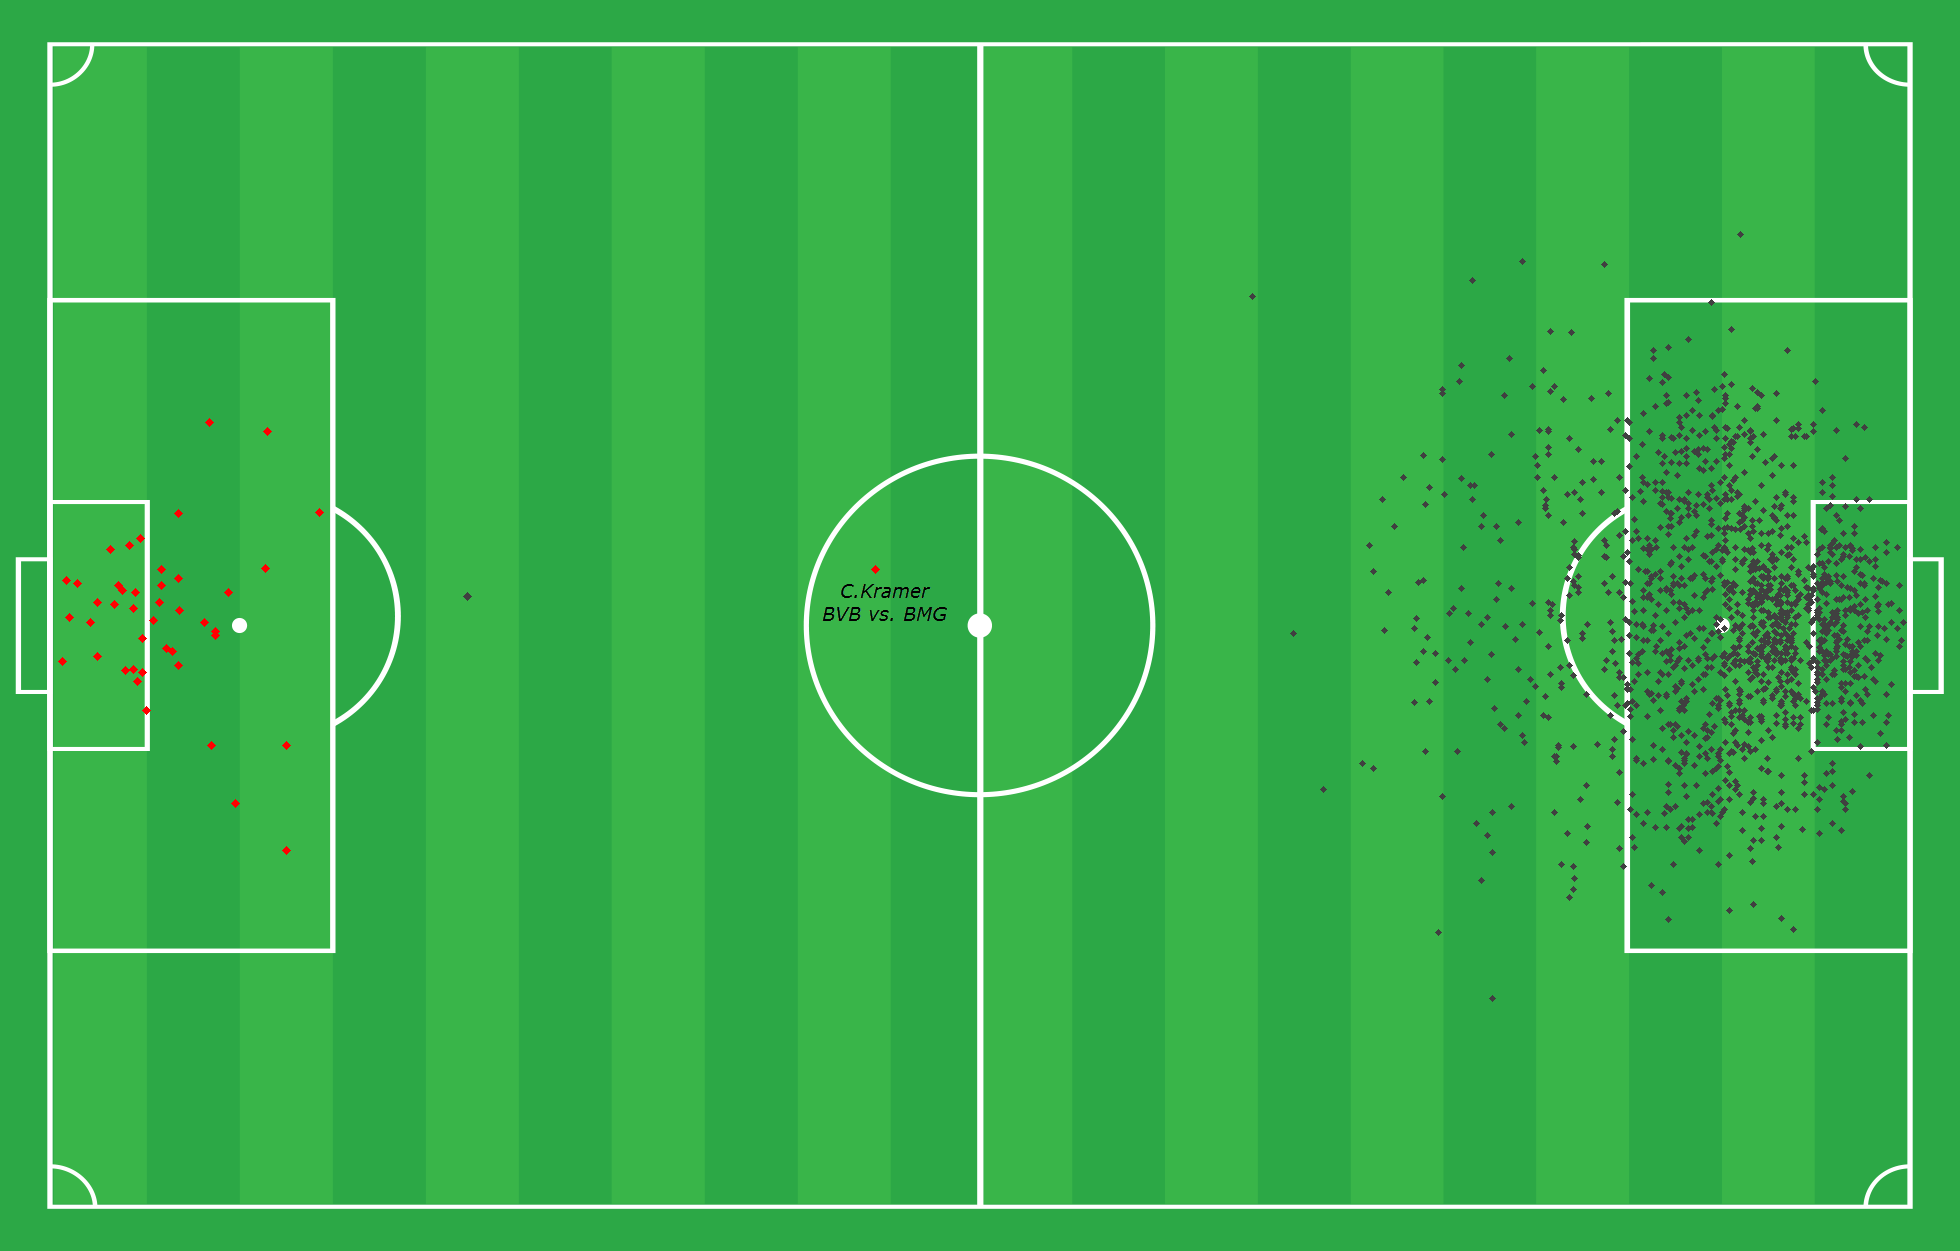
\includegraphics[scale=0.28]{se-wa-jpg/owngoals}
%\caption[Ausschluss der Eigentore]{Ausschluss der Eigentore}
%\label{owngoals}
%\end{figure}
